\section{The Philokalia’s Martial Character}

\begin{quotex}
What struck me on the beach--and it struck me indeed, so that I staggered as at a blow--was that if the Eternal Principle had rested in that curved thorn I had carried about my neck across so many leagues, and if it now rested in the new thorn (perhaps the same thorn) I had only now put there, then it might rest in everything, in every thorn in every bush, in every drop of water in the sea. The thorn was a sacred Claw because all thorns were sacred Claws; the sand in my boots was sacred sand because it came from a beach of sacred sand. The cenobites treasured up the relics of the sannyasins because the sannyasins had approached the Pancreator. But everything had approached and even touched the Pancreator, because everything had dropped from his hand. Everything was a relic. All the world was a relic. I drew off my boots, that had traveled with me so far, and threw them into the waves that I might not walk shod on holy ground.
\flright{\textsc{Gene Wolf}\footnote{\url{http://www.goodreads.com/author/quotes/23069.Gene\_Wolfe}}, \textit{Citadel of the Autarch}\footnote{\url{http://www.depauw.edu/sfs/interviews/wolfe46interview.htm}}}
\end{quotex}


\begin{wrapfigure}{rt}{.3\textwidth}
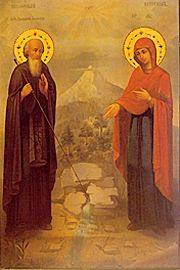
\includegraphics[width=.3\textwidth]{Athanasius_of_Athos.jpg}
\end{wrapfigure}

We've been given, as Christians, and have accepted, as fools, a very impoverished reading of Scripture, one in which Jesus emerges as someone so milquetoast\footnote{\url{http://en.wikipedia.org/wiki/Caspar\_Milquetoast}} that He wouldn't dare overturn the money-changing temples and bureaucratic stalls of Liberaldom or secular Democracy, could He by fickle mishap, arrive today. In a perverted sense, this is entirely true, for even this ``phase'' (degenerative as it may be), must exist entirely and utterly (though not \emph{self-consciously}) of His will, alone. As Cologero points out, this period of chaos must have Laws which govern it as well, just ones we're not as used to noticing. Yet, when the man comes around\footnote{\url{http://www.youtube.com/watch?v=k9IfHDi-2EA}}, the rules will get a lot less murky, quickly. There's a huge difference between God in heaven giving man time, and God descending to sort it out.

As for these difficult-to-discern-patterns of the Kali Yuga, could it be that part of the reason the Bourgeois Period is still alive and kicking is that ignorant men, latently of the brahminic or warrior caste, deliberately and desperately support it, seeing quite clearly the huge gap between the Third Estate epoch \& the epoch of the Shudra and the Outcast? After all, the merchant class is still ``objective'', at least; the Shudra is neither objective, nor free. Not seeing the huge gap between the Third Estate and that of their own (since it is unrealized), they volunteer to wage the struggle to stave off the tidal wave. This seems to be Mencius Moldbug's conclusion in this piece of punditry\footnote{\url{http://unqualified-reservations.blogspot.com/2013/06/civil-liberties-and-single-reactionary.html}}, for instance:

\begin{quotex}
Moreover, the fascist militarists who actually do this job are some of the best men in America. \textbf{American communism, for obvious reasons, loves to send America's best men to Afghanistan to get their private parts Osterized by fertilizer bombs}. This is American war since 1945: State solving the problem of how it can get DoD to stick its d--- in a blender. Solving it rather well, I'd say. Many of America's best men are in the Pentagon, and good men know how to obey, and into the blender goes that d---. Still, much testicle remains.
\end{quotex}


How long will the warrior caste (even more so those imitating it, either out of malice or virtue) be content with propping up a ``country'' designed to make life easy for the worst specimens of humanity? Now extending its obligation\footnote{\url{http://www.huffingtonpost.com/2013/06/28/obama-africa-hunger\_n\_3515684.html}} (and therefore, its power) to the entire planet? We shall see -- there are a lot of soldiers returning from the Middle East.

Also, it seems clear to me that the Spirit behind modern culture, for obvious reasons, wants to convince those who are formally, latently, or partially (if not truly) Good that Good and Evil are illusions, and that in the name of some catch-phrases like Equality \& Tolerance, Life ought to be made easier for everyone, even those who really aren't aware of anything above them, even their conscience. Isn't this what Evil would say to Good? That in reality, the distance between us is an Illusion? Something Jesus said comes to mind:

\begin{quotex}
And the lord commended the unjust steward, because he had done wisely: for the children of this world are in their generation wiser than the children of light. 
\flright{\textsc{Luke 16:8}}
\end{quotex}


Could it be that the Revolutionaries have long known (better than most) that seeing into the Nature of man is pre-requisite to changing things? Granted, they can only imagine that Good exists because of sluggish inertia, that it couldn't last, except as an inherited accretion and knee-jerk reflex (which of course, sees things backwards, given that most people engage in Evil for precisely this reason). But they have been adept\footnote{\url{http://en.wikipedia.org/wiki/Frantz\_Fanon}} at manipulating the remnants of the castes to achieve their end. Have you taken a literary criticism class, lately? All you read is literature of perversion and revolt. Take Sarah Kane\footnote{\url{http://en.wikipedia.org/wiki/Sarah\_Kane}}, for instance. Every effort is being made to extend the suffering of our ``elites'' through the ``middle'' and to unite that suffering with the lower castes. I saw a sign on a church recently which, against all odds, was actually apropos: ``While we play Church, God's creation becomes more corrupt.'' The Bible Belt itself is not as well off\footnote{\url{https://www.prbuzz.com/non-profit/70427-depression-and-pornography.html}} as it appears.

What would a Frankish noble have done if confronted with the modern world? Undoubtedly, after a tour through both prison and mental health facilities, he would have emerged much wiser and more cautious of General Law\footnote{\url{http://www.gornahoor.net/?tag=general-law}}. He would (in fact) lay plans with a prudence and cunning that would complement his innate qualities, and guarantee a larger success in the long run. On the other hand, the qualities he has innately, I lack. What can I learn from him, and where can I learn it? \emph{As noted above, there is the possibility of learning from our enemies, in that we see by negative example, how they employ means to ends and discern what is best for their kind}.

But there is much more for those who wish to transcend the purely Mephistophelean character of the clever Revolutionary, the spirit who negates\footnote{\url{http://www.pointandcircumference.com/macropoetics/Dante.htm}}, the composting bacteria which works among those whose souls die before they ever learned they had them:

\begin{quotex}
With Faust, the Romantic rebellion breaks out in full force. At the outset, the poem promises to take the reader ``from Heaven through the world to Hell.'' Note the inverse direction. And still less than Paradise Lost does Faust portray a coherent universe. A scene in a student hangout, a seduction drama, the spectacles of the first and second Walpurgisnacht, Faust's adventures as general, artist and civil-engineer-cum-dictator -- all this does not add up to a comprehensive portrayal of human life. The flames of Hell, briefly glimpsed, are taken about as seriously as in a comic strip; while Heaven (complete with a ``old guy'' Deity at whom the urbane and sophisticated devil thumbs his nose) is but the self-serving reflection of a middle world where the amoral have their way. \textbf{Unlike Dante's journey, Faust's is the opposite of instructive}. At the end the hero has destroyed the world and learned nothing, the angels confuse his ruthlessness with aspiration; and the author himself seems to have \emph{unlearned} whatever awareness of right and wrong he may have had at the outset. The final scene of {Faust} appears meant to contradict the scene at the summit of Purgatory where Beatrice insists on confronting Dante with his peccadilloes: ``A high law of G-d would be broken if Lethe were passed and such food tasted without some toll of remorse that sheds tears.'' Faust does not have to say he is sorry; enters heaven in the company of \emph{unborn children,} consciousness and conscience are effaced. The Israeli scholar Rivkah Schechter is, I believe, right in seeing Faust as the prelude to Auschwitz.
\end{quotex}


Hence, we turn to very particular texts, spiritual and literary and political, to nourish the awareness which we lack, which we horn-swoggled ourselves out of by accepting the Devil's food when we should have been vigilant.

\begin{quotex}
Law: mechanism which should be used in whatever way will generate the preferred result. Old fashioned law did too much to protect individuals from the social will. the mediocratic model avoids bourgeois notions such as principles or liberties. If the community believes someone should be punished, the legal system should not put obstacles in the way. The idea of providing protection for defendants from the state is no longer required, as modern state agents can be presumed to act on behalf of society rather than on behalf of an elite. \textbf{Mediocracy believes in having as many laws as possible, but enforcing them selectively. This provides maximum flexibility, since harassment can be targeted at appropriate individuals.} 
\flright{\textsc{Fabian Tassano}, \textit{Mediocracy}}
\end{quotex}


Christ the King told Satan to ``get thee behind me'' during the Temptation, which was the rough equivalent of a medieval king saying ``away with you, you varlet!''. Then, and only then, did angels minister to him. One of the traditional Christian's first tasks will be to learn not to accept a part in the inverted medieval passion play of the Spirit of the Age, but rather to wrestle with the powers and principalities (within himself, foremost) and force them to play the role in his own mystery play. For those ``waking up'', seemingly innocuous things take on spiritual significance. They ``manifest''. Do we wish to become cardboard characters, doomed to fire, in his play, or force him to step into our own?

Isn't this the root of the ``difficulty with Christianity''? Is it what it appears to be? It may look milquetoast, but this is an illusion. The regal-warrior spirit is carefully hidden in plain sight. Christ becomes a King by rejecting the world, the flesh, and the devil, by repulsing Satan's attempt to get him to play a part in a play in which his lines were penned by Satan. Isn't this what the Revolutionary narrative is all about? We may not know all, or even much, but we know \emph{enough}. Enough to begin to resist the temptation.

Spirituality such as found in the \emph{Philokalia} nourished the spiritual life of the Eastern Empire, \& from them, flowed westward, even if indirectly\footnote{\url{http://en.wikipedia.org/wiki/The\_Cloud\_of\_Unknowing}}. The Franks gladly submitted to the High King of Heaven: Chlodovechus exclaimed ``Oh, if I had been there with my Franks!''\footnote{\url{http://books.google.com/books?id=maMXAAAAYAAJ&pg=PA11&lpg=PA11&dq=had+I+been+there+with+my+franks&source=bl&ots=s2TTKEM_i4&sig=2KwFfrp1sd3jJHONKYTErse9aK4&hl=en&sa=X&ei=JFzMUfPuHcS1ygHmvIDABQ&ved=0CEUQ6AEwBA\#v=onepage&q=had\%20I\%20been\%20there\%20with\%20my\%20franks&f=false}}. It's possible to view this as an aberration and twisting of Aryan spirituality. But then, what do you do with such organizations as this\footnote{\url{http://en.wikipedia.org/wiki/Iron\_Guard}}? What about the Templars? Together, the Western tribes and the religion of Christianity created a fuller manifestation of Tradition (and corresponding higher aberrations, at times, when corrupt) than possible otherwise. \emph{Corruptio optima pessimi}.


Here is practical advice from the \emph{Philokalia} -- it has the smell of authenticity, as it isn't something one would ``make up'' on the spur of the moment. If one isn't a Brahmin, then simply gain the appropriate insight and apply it to your own circumstances. For instance, knowing that some thoughts have a demonic origin is highly useful, no matter what caste you belong to. I think you will see that this corpus of spiritual teaching is anything but ``sentimental'' and ``Semitic''. It is, in fact, triumphant and almost Promethean.

\begin{quotationx}
Similarly, anger, whether reasonable or unreasonable, obstructs our spiritual vision. Our incensive power can be used in a way that is according to nature only when turned against our own impassioned or self-indulgent thoughts. We must not therefore expend all our effort in bodily fasting; we must also give attention to our thoughts and to spiritual meditation, since otherwise we will not be able to advance to the heights of true purity and chastity.

If a man, still enmeshed in sin and anger, dares shamelessly to reach out for knowledge of divine things, or even to embark upon immaterial prayer, he deserves the rebuke given by the Apostle; for it is dangerous for him to pray with head bare and uncovered. Such a soul, he says, ought to `have a veil on her head because of the angels' (cf I Cor. 11:5-7), and to be clothed in due reverence and humility.

Blessed is the monk who regards every man as God after God.

There are times when the demons suggest thoughts to you and then urge you to rebut them with prayer; whereupon they withdraw of their own accord, so as to deceive you into imagining that you have begun to overcome such thoughts and to rout the demons.

You should be aware of this trick: at times the demons split into two groups; and when you call for help against one group, the other will come in the guise of angels and drive away the first, so that you are deceived into believing that they are truly angels.

When the intellect attains prayer that is pure and free from passion, the demons attack no longer with sinister thoughts but with thoughts of what is good. For they suggest to it an illusion of God's glory in a form pleasing to the senses, so as to make it think that it has realized the final aim of prayer. A man who possesses spiritual knowledge has said that this illusion results from the passion of self-esteem and from the demon's touch upon a certain area of the brain.

Know that the holy angels encourage us to pray and stand beside us, rejoicing and praying for us (cf Tobit 12:12). Therefore, if we are negligent and admit thoughts from the enemy, we greatly provoke the angels. For while they struggle hard on our behalf we do not even take the trouble to pray to God for ourselves, but we despise their services to us, and, abandoning their Lord and God, we consort with unclean demons.

One who has attained dispassion has not necessarily achieved pure prayer. For he may still be occupied with thoughts which, though dispassionate, distract him and keep him far from God.

Undistracted prayer is the highest intellection of the intellect.

The warfare between us and the demons is waged solely on account of spiritual prayer; for prayer is extremely hateful and offensive to them, whereas it leads us to salvation and peace.

When the intellect has been perfected, it unites wholly with God and is illumined by divine light, and the most hidden mysteries are revealed to it. Then it truly learns where wisdom and power lie... While it is still fighting against the passions it cannot as yet enjoy these things... But once the battle is over and it is found worthy of spiritual gifts, then it becomes wholly luminous, powerfully energized by grace and rooted in the contemplation of spiritual realities. A person in whom this happens is not attached to the things of this world but has passed from death to life.
\end{quotationx}


Ironically, there is a ``martial'' quality about the \emph{Philokalia}, which is consonant with the ``marching character'' of Christianity, itself a religion (in many ways) that was military. The Church, after all, was ``militant''. If it was\footnote{\url{http://riversfromeden.wordpress.com/2012/04/20/christians-in-the-roman-army-countering-the-pacifist-narrative/}} (perhaps dubitably) a religion of the lower castes, nevertheless, it should be remembered that it was through the Roman army \& Constantine, ultimately, that the religion won its victory over those, like Julian the Apostate, who wished to endorse Iamblichus and the NeoPlatonists rather than a religion. Christianity ``chose sides'' because it has a martial quality. I think this is the way to ``resolve'' the debate with neo-pagans: the Vedantic wing of Christianity wasn't strong enough to preclude an all-out war against all ``paganism'', so perhaps this should be rectified.

Yet Christ is a King, not merely a high priest. And the King is not mocked; He is no sentimentalist, but like a detached general, he awaits the inevitable outcome of His warfare. The King is Dead. Long live the King. The King is Coming. Life itself, the King.

\begin{quotex}
We believe that we invent symbols. The truth is that they invent us; we are their creatures, shaped by their hard, defining edges. When soldiers take their oath they are given a coin, an asimi stamped with the profile of the Autarch. Their acceptance of that coin is their acceptance of the special duties and burdens of military life---they are soldiers from that moment, though they may know nothing of the management of arms. I did not know that then, but it is a profound mistake to believe that we must know of such things to be influenced by them, and in fact to believe so is to believe in the most debased and superstitious kind of magic. The would-be sorcerer alone has faith in the efficacy of pure knowledge; rational people know that things act of themselves or not at all.

\flright{\textsc{Gene Wolfe}\footnote{\url{http://www.goodreads.com/author/show/23069.Gene\_Wolfe}}, \emph{Shadow and Claw}\footnote{\url{http://www.goodreads.com/work/quotes/40575}}}
\end{quotex}


The ``Third Wave'' of Christianity will come when Christians themselves reclaim their monarchic legacy, hidden in Scripture, of Christ as the prophet, priest, and king (warrior). If we apply the insights of the Philokalia quoted above, we would conclude that the history of the West has been a very careful, selective seducement of a predominantly warrior-religion, designed to ``set it up'' for a final illusion. That is, the glories of the Renaissance and the wonders of Science and the blessed peace of secular humanism are analogous to demonically-induced spiritual states designed to convince the one who undergoes them that they are ``favored'' and have reached ``deliverance''. However, there is still a chance that the victory of Logos in the West can be redeemed. That is, instead of the Divine withdrawing back into the Divine, the human can be drawn up into God (the aim of Christian warfare, which approaches the passions with warfare in an attempt to ``possess'' them for God). This can only happen if the West uses discernment to see that the Logos presented to it, of which it is most acutely aware, is to be sanctified to God \& taken up.

Thus, Western Christians have to see, at one and the same time, both the limitations of its Tradition (a warrior-religion) and the timelessness of it (a true reflection of something Transcendent, which was worth defending, albeit with more wisdom). This will involve restoring the ``Vedantic wing'' of the Faith, which will include esoteric studies. All resurgencies, ill-fated or blessed, of Christianity have begun with the return to ``Christ the King''.


\flrightit{Posted on 2013-07-05 by Logres}

\begin{center}* * *\end{center}

\begin{footnotesize}
\begin{sffamily}
\texttt{michel on 2013-07-06 at 10:39 said:}

Yes! If only more elites were like you Logres, then the restoration greatly longed for might stand a chance. I pray that the vigor of your writing is reflected in your actions.

\hfill

\texttt{Jason-Adam on 2013-07-06 at 12:26 said:}

This is amazing. I am inwardly in a similar state of being as Logres; independently I had come to the same conclusion myself that true, mediaeval Christianity was and is a militant, intolerant, warrior religion that gives to the man who follows it a high will to power and dominance, the ability to control his emotions, and a sense of community that gives the fight of our life meaning and purpose that transcends not only ourselves but all time and space... ... ... ... .

\hfill

\texttt{Logres on 2013-07-06 at 22:14 said:}

Thank you both for reading, although I am not one of the current elites (for which I begin to be more thankful, the more I learn). I wrote this partly because several readers last year had asked ``what to do?'', wondering if Christianity had anything to offer. I think, after reading in the Philokalia, that it does, \& have been pointed back to the theme of invisible warfare. Who would this NOT help? I am also glad that others perceive this too -- which makes neo-pagan denial of Medieval tradition all the more... well, odd. Thank you for your prayers, Michael.

\hfill

\texttt{Jason-Adam on 2013-07-08 at 12:56 said:}

Dear Logres,

may I ask do you have a personal regimen of spiritual practice ? I apologise if this sounds rude but as I see that we are similar minds though you seem to be of a higher level of development, I ask because I'd like to learn from you.

Also, have you read this book before ? It's Orthodox and ant-Catholic so I have some issues with it but all in all it makes a good defence of monarchy and the mediaeval Christian Tradition.

\url{http://www.romanitas.ru/eng/THE\%20MYSTERY\%20OF\%20CHRISTIAN\%20POWER.htm}


Lastly, in the past you've discussed Franz Bardon, would you recommend his books and exercises for someone looking for a transcendent experience ?

\hfill

\texttt{Logres on 2013-07-10 at 11:38 said:}

Jason, I think ``intolerant'' here is certainly in the sense of the modern word. That is, Christianity has no room for any competing -isms, heresies, etc., and maintains a traditional character, period. It is not interested in accomodating anything at the cost of its principles, although it may stoop in charity, infinitely. And it would certainly resist (if it were strong) incursions from foreign bodies who were designing to feed off its corpse (eg., modern Islam, the full blown Reformation political movement, etc.).

\hfill

\end{sffamily}
\end{footnotesize}

